\chapter{Multi-planar Reconstruction}
\vspace{-10mm}
\label{multiplanar}

Multi-planar Reconstruction (MPR) in medical imaging is a way of displaying three-dimensional images, captured on an imaging device. A three-dimensional study is displayed in three orthogonal slices. In each slice, there are indicated positions of the other two slices - each slice includes two lines giving the positions (See Figure \ref{fig:multiplanar}). The slices are most often parallel to basic anatomy planes\cite{ctteachingmanual}: sagittal, coronal and transverse plane.  Implementation of Multi-planar Reconstruction was requested by IKEM.

\begin{figure}
 	\caption{Multi-planar reconstruction in Dicom-Presenter.\label{fig:multiplanar}}
	\begin{center}
	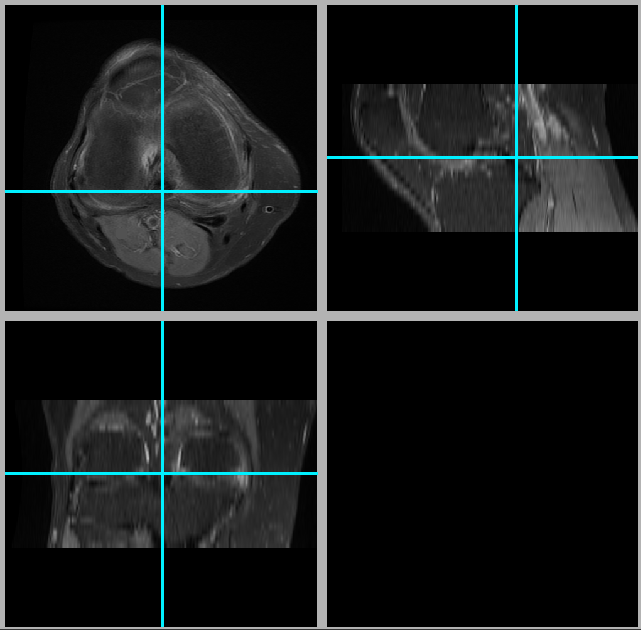
\includegraphics[width=0.75\textwidth]{Text/IMG/MultiPlanar.png}
	\end{center}
\end{figure}

\section{Implementation of Multi-planar Reconstruction}

An implementation of MPR could be divided into three parts:

\begin{itemize}
\item Handling user control. %User has to be able to freely manipulate with the three planes. Is existing
\item Image Rendering. %Is it possible to use existing classes to render three planes of a DICOM study?
\item Integration to existing object model. %The questions are, where to place the new class in the existing class hierarchy (see Section \ref{dpobjectmodel}) and how much functionality of the new class can be inherited from existing classes.
\end{itemize}

The question to discuss in all three steps is, how much of existing functionality can be used and what parts are necessary to be implemented. It is possible to implement a completely new class, which will handle user control and rendering itself. But it would lead to multiple implementations of similar tasks. The aim is to use maximum of existing functionality.

The functionality of new classes performing Multi-planar reconstruction will be similar to existing classes: Workspace and Image. Workspace class manages placement of images on the computer screen - similarly, three slices of MPR will be placed on computer screen. There is a process of obtaining proper slice from a three-dimensional image in the Image class. When using MPR, three slices will be taken in three orthogonal planes.

The similarities to Image and Workspace class could be solved in three ways:

\begin{itemize}
\item It is possible to create a new standalone class, which will have partially similar functionality to the existing one.
\item The new functionality can be added to the existing class.
\item An identical functionality of the class and existing class can be extracted into an abstract class, which will be inherited by both of them.
\end{itemize}


